\documentclass[1p]{elsarticle_modified}
%\bibliographystyle{elsarticle-num}

%\usepackage[colorlinks]{hyperref}
%\usepackage{abbrmath_seonhwa} %\Abb, \Ascr, \Acal ,\Abf, \Afrak
\usepackage{amsfonts}
\usepackage{amssymb}
\usepackage{amsmath}
\usepackage{amsthm}
\usepackage{scalefnt}
\usepackage{amsbsy}
\usepackage{kotex}
\usepackage{caption}
\usepackage{subfig}
\usepackage{color}
\usepackage{graphicx}
\usepackage{xcolor} %% white, black, red, green, blue, cyan, magenta, yellow
\usepackage{float}
\usepackage{setspace}
\usepackage{hyperref}

\usepackage{tikz}
\usetikzlibrary{arrows}

\usepackage{multirow}
\usepackage{array} % fixed length table
\usepackage{hhline}

%%%%%%%%%%%%%%%%%%%%%
\makeatletter
\renewcommand*\env@matrix[1][\arraystretch]{%
	\edef\arraystretch{#1}%
	\hskip -\arraycolsep
	\let\@ifnextchar\new@ifnextchar
	\array{*\c@MaxMatrixCols c}}
\makeatother %https://tex.stackexchange.com/questions/14071/how-can-i-increase-the-line-spacing-in-a-matrix
%%%%%%%%%%%%%%%

\usepackage[normalem]{ulem}

\newcommand{\msout}[1]{\ifmmode\text{\sout{\ensuremath{#1}}}\else\sout{#1}\fi}
%SOURCE: \msout is \stkout macro in https://tex.stackexchange.com/questions/20609/strikeout-in-math-mode

\newcommand{\cancel}[1]{
	\ifmmode
	{\color{red}\msout{#1}}
	\else
	{\color{red}\sout{#1}}
	\fi
}

\newcommand{\add}[1]{
	{\color{blue}\uwave{#1}}
}

\newcommand{\replace}[2]{
	\ifmmode
	{\color{red}\msout{#1}}{\color{blue}\uwave{#2}}
	\else
	{\color{red}\sout{#1}}{\color{blue}\uwave{#2}}
	\fi
}

\newcommand{\Sol}{\mathcal{S}} %segment
\newcommand{\D}{D} %diagram
\newcommand{\A}{\mathcal{A}} %arc


%%%%%%%%%%%%%%%%%%%%%%%%%%%%%5 test

\def\sl{\operatorname{\textup{SL}}(2,\Cbb)}
\def\psl{\operatorname{\textup{PSL}}(2,\Cbb)}
\def\quan{\mkern 1mu \triangleright \mkern 1mu}

\theoremstyle{definition}
\newtheorem{thm}{Theorem}[section]
\newtheorem{prop}[thm]{Proposition}
\newtheorem{lem}[thm]{Lemma}
\newtheorem{ques}[thm]{Question}
\newtheorem{cor}[thm]{Corollary}
\newtheorem{defn}[thm]{Definition}
\newtheorem{exam}[thm]{Example}
\newtheorem{rmk}[thm]{Remark}
\newtheorem{alg}[thm]{Algorithm}

\newcommand{\I}{\sqrt{-1}}
\begin{document}

%\begin{frontmatter}
%
%\title{Boundary parabolic representations of knots up to 8 crossings}
%
%%% Group authors per affiliation:
%\author{Yunhi Cho} 
%\address{Department of Mathematics, University of Seoul, Seoul, Korea}
%\ead{yhcho@uos.ac.kr}
%
%
%\author{Seonhwa Kim} %\fnref{s_kim}}
%\address{Center for Geometry and Physics, Institute for Basic Science, Pohang, 37673, Korea}
%\ead{ryeona17@ibs.re.kr}
%
%\author{Hyuk Kim}
%\address{Department of Mathematical Sciences, Seoul National University, Seoul 08826, Korea}
%\ead{hyukkim@snu.ac.kr}
%
%\author{Seokbeom Yoon}
%\address{Department of Mathematical Sciences, Seoul National University, Seoul, 08826,  Korea}
%\ead{sbyoon15@snu.ac.kr}
%
%\begin{abstract}
%We find all boundary parabolic representation of knots up to 8 crossings.
%
%\end{abstract}
%\begin{keyword}
%    \MSC[2010] 57M25 
%\end{keyword}
%
%\end{frontmatter}

%\linenumbers
%\tableofcontents
%
\newcommand\colored[1]{\textcolor{white}{\rule[-0.35ex]{0.8em}{1.4ex}}\kern-0.8em\color{red} #1}%
%\newcommand\colored[1]{\textcolor{white}{ #1}\kern-2.17ex	\textcolor{white}{ #1}\kern-1.81ex	\textcolor{white}{ #1}\kern-2.15ex\color{red}#1	}

{\Large $\underline{12a_{0814}~(K12a_{0814})}$}

\setlength{\tabcolsep}{10pt}
\renewcommand{\arraystretch}{1.6}
\vspace{1cm}\begin{tabular}{m{100pt}>{\centering\arraybackslash}m{274pt}}
\multirow{5}{120pt}{
	\centering
	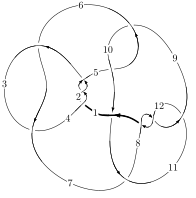
\includegraphics[width=112pt]{../../../GIT/diagram.site/Diagrams/png/1615_12a_0814.png}\\
\ \ \ A knot diagram\footnotemark}&
\allowdisplaybreaks
\textbf{Linearized knot diagam} \\
\cline{2-2}
 &
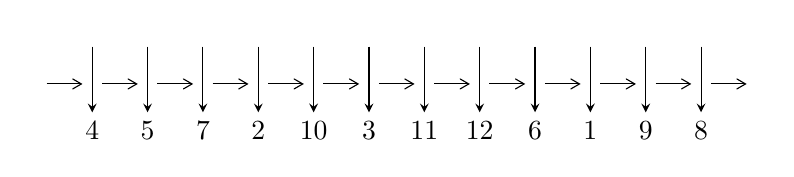
\begin{tikzpicture}[x=20pt, y=17pt]
	% nodes
	\node (C0) at (0, 0) {};
	\node (C1) at (1, 0) {};
	\node (C1U) at (1, +1) {};
	\node (C1D) at (1, -1) {4};

	\node (C2) at (2, 0) {};
	\node (C2U) at (2, +1) {};
	\node (C2D) at (2, -1) {5};

	\node (C3) at (3, 0) {};
	\node (C3U) at (3, +1) {};
	\node (C3D) at (3, -1) {7};

	\node (C4) at (4, 0) {};
	\node (C4U) at (4, +1) {};
	\node (C4D) at (4, -1) {2};

	\node (C5) at (5, 0) {};
	\node (C5U) at (5, +1) {};
	\node (C5D) at (5, -1) {10};

	\node (C6) at (6, 0) {};
	\node (C6U) at (6, +1) {};
	\node (C6D) at (6, -1) {3};

	\node (C7) at (7, 0) {};
	\node (C7U) at (7, +1) {};
	\node (C7D) at (7, -1) {11};

	\node (C8) at (8, 0) {};
	\node (C8U) at (8, +1) {};
	\node (C8D) at (8, -1) {12};

	\node (C9) at (9, 0) {};
	\node (C9U) at (9, +1) {};
	\node (C9D) at (9, -1) {6};

	\node (C10) at (10, 0) {};
	\node (C10U) at (10, +1) {};
	\node (C10D) at (10, -1) {1};

	\node (C11) at (11, 0) {};
	\node (C11U) at (11, +1) {};
	\node (C11D) at (11, -1) {9};

	\node (C12) at (12, 0) {};
	\node (C12U) at (12, +1) {};
	\node (C12D) at (12, -1) {8};
	\node (C13) at (13, 0) {};

	% arrows
	\draw[->,>={angle 60}]
	(C0) edge (C1) (C1) edge (C2) (C2) edge (C3) (C3) edge (C4) (C4) edge (C5) (C5) edge (C6) (C6) edge (C7) (C7) edge (C8) (C8) edge (C9) (C9) edge (C10) (C10) edge (C11) (C11) edge (C12) (C12) edge (C13) ;	\draw[->,>=stealth]
	(C1U) edge (C1D) (C2U) edge (C2D) (C3U) edge (C3D) (C4U) edge (C4D) (C5U) edge (C5D) (C6U) edge (C6D) (C7U) edge (C7D) (C8U) edge (C8D) (C9U) edge (C9D) (C10U) edge (C10D) (C11U) edge (C11D) (C12U) edge (C12D) ;
	\end{tikzpicture} \\
\hhline{~~} \\& 
\textbf{Solving Sequence} \\ \cline{2-2} 
 &
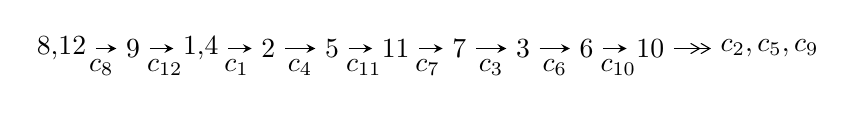
\begin{tikzpicture}[x=23pt, y=7pt]
	% node
	\node (A0) at (-1/8, 0) {8,12};
	\node (A1) at (1, 0) {9};
	\node (A2) at (33/16, 0) {1,4};
	\node (A3) at (25/8, 0) {2};
	\node (A4) at (33/8, 0) {5};
	\node (A5) at (41/8, 0) {11};
	\node (A6) at (49/8, 0) {7};
	\node (A7) at (57/8, 0) {3};
	\node (A8) at (65/8, 0) {6};
	\node (A9) at (73/8, 0) {10};
	\node (C1) at (1/2, -1) {$c_{8}$};
	\node (C2) at (3/2, -1) {$c_{12}$};
	\node (C3) at (21/8, -1) {$c_{1}$};
	\node (C4) at (29/8, -1) {$c_{4}$};
	\node (C5) at (37/8, -1) {$c_{11}$};
	\node (C6) at (45/8, -1) {$c_{7}$};
	\node (C7) at (53/8, -1) {$c_{3}$};
	\node (C8) at (61/8, -1) {$c_{6}$};
	\node (C9) at (69/8, -1) {$c_{10}$};
	\node (A10) at (11, 0) {$c_{2},c_{5},c_{9}$};

	% edge
	\draw[->,>=stealth]	
	(A0) edge (A1) (A1) edge (A2) (A2) edge (A3) (A3) edge (A4) (A4) edge (A5) (A5) edge (A6) (A6) edge (A7) (A7) edge (A8) (A8) edge (A9) ;
	\draw[->>,>={angle 60}]	
	(A9) edge (A10);
\end{tikzpicture} \\ 

\end{tabular} \\

\footnotetext{
The image of knot diagram is generated by the software ``\textbf{Draw programme}" developed by Andrew Bartholomew(\url{http://www.layer8.co.uk/maths/draw/index.htm\#Running-draw}), where we modified some parts for our purpose(\url{https://github.com/CATsTAILs/LinksPainter}).
}\phantom \\ \newline 
\centering \textbf{Ideals for irreducible components\footnotemark of $X_{\text{par}}$} 
 
\begin{align*}
I^u_{1}&=\langle 
9.56930\times10^{26} u^{91}+4.97491\times10^{26} u^{90}+\cdots+1.83397\times10^{27} b+3.92664\times10^{27},\\
\phantom{I^u_{1}}&\phantom{= \langle  }-5.52127\times10^{26} u^{91}-8.62278\times10^{26} u^{90}+\cdots+1.83397\times10^{27} a-2.61403\times10^{27},\;u^{92}-4 u^{91}+\cdots-8 u^2+1\rangle \\
I^u_{2}&=\langle 
b- u-1,\;u^2+a+u+3,\;u^3+2 u-1\rangle \\
I^u_{3}&=\langle 
- u^2 a- u^2+b+u-1,\;- u^2 a+a^2+2 a u- u^2- a+2 u-3,\;u^3- u^2+2 u-1\rangle \\
I^u_{4}&=\langle 
b- u-1,\;- u^3- u^2+a- u-1,\;u^4+u^3+2 u^2+2 u+1\rangle \\
\\
\end{align*}
\raggedright * 4 irreducible components of $\dim_{\mathbb{C}}=0$, with total 105 representations.\\
\footnotetext{All coefficients of polynomials are rational numbers. But the coefficients are sometimes approximated in decimal forms when there is not enough margin.}
\newpage
\renewcommand{\arraystretch}{1}
\centering \section*{I. $I^u_{1}= \langle 9.57\times10^{26} u^{91}+4.97\times10^{26} u^{90}+\cdots+1.83\times10^{27} b+3.93\times10^{27},\;-5.52\times10^{26} u^{91}-8.62\times10^{26} u^{90}+\cdots+1.83\times10^{27} a-2.61\times10^{27},\;u^{92}-4 u^{91}+\cdots-8 u^2+1 \rangle$}
\flushleft \textbf{(i) Arc colorings}\\
\begin{tabular}{m{7pt} m{180pt} m{7pt} m{180pt} }
\flushright $a_{8}=$&$\begin{pmatrix}1\\0\end{pmatrix}$ \\
\flushright $a_{12}=$&$\begin{pmatrix}0\\u\end{pmatrix}$ \\
\flushright $a_{9}=$&$\begin{pmatrix}1\\u^2\end{pmatrix}$ \\
\flushright $a_{1}=$&$\begin{pmatrix}- u\\u\end{pmatrix}$ \\
\flushright $a_{4}=$&$\begin{pmatrix}0.301056 u^{91}+0.470171 u^{90}+\cdots-2.96443 u+1.42534\\-0.521781 u^{91}-0.271265 u^{90}+\cdots-1.81529 u-2.14106\end{pmatrix}$ \\
\flushright $a_{2}=$&$\begin{pmatrix}0.132509 u^{91}+1.28972 u^{90}+\cdots-1.42156 u+1.98262\\-1.74961 u^{91}+3.41466 u^{90}+\cdots-2.45957 u-2.11975\end{pmatrix}$ \\
\flushright $a_{5}=$&$\begin{pmatrix}0.499637 u^{91}-3.19051 u^{90}+\cdots-2.69354 u-1.70145\\1.20761 u^{91}-2.29856 u^{90}+\cdots+2.49070 u+0.858623\end{pmatrix}$ \\
\flushright $a_{11}=$&$\begin{pmatrix}u\\u^3+u\end{pmatrix}$ \\
\flushright $a_{7}=$&$\begin{pmatrix}- u^4- u^2+1\\- u^6-2 u^4- u^2\end{pmatrix}$ \\
\flushright $a_{3}=$&$\begin{pmatrix}0.133234 u^{91}-0.329272 u^{90}+\cdots-4.03448 u-0.614475\\-0.164836 u^{91}+0.0117691 u^{90}+\cdots-0.440981 u-0.836998\end{pmatrix}$ \\
\flushright $a_{6}=$&$\begin{pmatrix}0.500057 u^{91}-1.31833 u^{90}+\cdots-1.15620 u+0.817075\\-0.663481 u^{91}+0.793381 u^{90}+\cdots-0.361576 u-1.01523\end{pmatrix}$ \\
\flushright $a_{10}=$&$\begin{pmatrix}u^5+2 u^3+u\\- u^5- u^3+u\end{pmatrix}$\\&\end{tabular}
\flushleft \textbf{(ii) Obstruction class $= -1$}\\~\\
\flushleft \textbf{(iii) Cusp Shapes $= \frac{2365091250833776522114268693}{916983961196051693206135667} u^{91}-\frac{18729853830167391906229939375}{1833967922392103386412271334} u^{90}+\cdots-\frac{1024932205509583481893242009}{1833967922392103386412271334} u-\frac{16203344775728881724174542717}{1833967922392103386412271334}$}\\~\\
\newpage\renewcommand{\arraystretch}{1}
\flushleft \textbf{(iv) u-Polynomials at the component}\newline \\
\begin{tabular}{m{50pt}|m{274pt}}
Crossings & \hspace{64pt}u-Polynomials at each crossing \\
\hline $$\begin{aligned}c_{1},c_{2},c_{4}\end{aligned}$$&$\begin{aligned}
&u^{92}-11 u^{91}+\cdots+10 u+1
\end{aligned}$\\
\hline $$\begin{aligned}c_{3},c_{6}\end{aligned}$$&$\begin{aligned}
&u^{92}+4 u^{91}+\cdots-576 u-128
\end{aligned}$\\
\hline $$\begin{aligned}c_{5},c_{9}\end{aligned}$$&$\begin{aligned}
&u^{92}+2 u^{91}+\cdots-352 u-64
\end{aligned}$\\
\hline $$\begin{aligned}c_{7}\end{aligned}$$&$\begin{aligned}
&u^{92}+4 u^{91}+\cdots-228 u+36
\end{aligned}$\\
\hline $$\begin{aligned}c_{8},c_{11},c_{12}\end{aligned}$$&$\begin{aligned}
&u^{92}-4 u^{91}+\cdots-8 u^2+1
\end{aligned}$\\
\hline $$\begin{aligned}c_{10}\end{aligned}$$&$\begin{aligned}
&u^{92}-20 u^{91}+\cdots-102752 u+13633
\end{aligned}$\\
\hline
\end{tabular}\\~\\
\newpage\renewcommand{\arraystretch}{1}
\flushleft \textbf{(v) Riley Polynomials at the component}\newline \\
\begin{tabular}{m{50pt}|m{274pt}}
Crossings & \hspace{64pt}Riley Polynomials at each crossing \\
\hline $$\begin{aligned}c_{1},c_{2},c_{4}\end{aligned}$$&$\begin{aligned}
&y^{92}-89 y^{91}+\cdots-208 y+1
\end{aligned}$\\
\hline $$\begin{aligned}c_{3},c_{6}\end{aligned}$$&$\begin{aligned}
&y^{92}-54 y^{91}+\cdots-716800 y+16384
\end{aligned}$\\
\hline $$\begin{aligned}c_{5},c_{9}\end{aligned}$$&$\begin{aligned}
&y^{92}+42 y^{91}+\cdots-25600 y+4096
\end{aligned}$\\
\hline $$\begin{aligned}c_{7}\end{aligned}$$&$\begin{aligned}
&y^{92}+4 y^{91}+\cdots+8856 y+1296
\end{aligned}$\\
\hline $$\begin{aligned}c_{8},c_{11},c_{12}\end{aligned}$$&$\begin{aligned}
&y^{92}+84 y^{91}+\cdots-16 y+1
\end{aligned}$\\
\hline $$\begin{aligned}c_{10}\end{aligned}$$&$\begin{aligned}
&y^{92}+28 y^{91}+\cdots+10518208240 y+185858689
\end{aligned}$\\
\hline
\end{tabular}\\~\\
\newpage\flushleft \textbf{(vi) Complex Volumes and Cusp Shapes}
$$\begin{array}{c|c|c}  
\text{Solutions to }I^u_{1}& \I (\text{vol} + \sqrt{-1}CS) & \text{Cusp shape}\\
 \hline 
\begin{aligned}
u &= -0.142365 + 1.052150 I \\
a &= \phantom{-}0.00718 + 2.51345 I \\
b &= \phantom{-}0.224624 - 1.256470 I\end{aligned}
 & -1.67872 + 2.40443 I & \phantom{-0.000000 } 0 \\ \hline\begin{aligned}
u &= -0.142365 - 1.052150 I \\
a &= \phantom{-}0.00718 - 2.51345 I \\
b &= \phantom{-}0.224624 + 1.256470 I\end{aligned}
 & -1.67872 - 2.40443 I & \phantom{-0.000000 } 0 \\ \hline\begin{aligned}
u &= -0.031893 + 1.093450 I \\
a &= \phantom{-}0.789128 + 0.767645 I \\
b &= -1.344780 - 0.179061 I\end{aligned}
 & \phantom{-}0.0460196 + 0.0531118 I & \phantom{-0.000000 } 0 \\ \hline\begin{aligned}
u &= -0.031893 - 1.093450 I \\
a &= \phantom{-}0.789128 - 0.767645 I \\
b &= -1.344780 + 0.179061 I\end{aligned}
 & \phantom{-}0.0460196 - 0.0531118 I & \phantom{-0.000000 } 0 \\ \hline\begin{aligned}
u &= -0.227106 + 1.094750 I \\
a &= -0.204440 + 0.030157 I \\
b &= \phantom{-}0.889203 + 0.208382 I\end{aligned}
 & \phantom{-}0.63573 + 4.55193 I & \phantom{-0.000000 } 0 \\ \hline\begin{aligned}
u &= -0.227106 - 1.094750 I \\
a &= -0.204440 - 0.030157 I \\
b &= \phantom{-}0.889203 - 0.208382 I\end{aligned}
 & \phantom{-}0.63573 - 4.55193 I & \phantom{-0.000000 } 0 \\ \hline\begin{aligned}
u &= -0.343914 + 1.068750 I \\
a &= \phantom{-}0.718999 - 1.078310 I \\
b &= -1.331240 - 0.090187 I\end{aligned}
 & -5.38660 + 7.98182 I & \phantom{-0.000000 } 0 \\ \hline\begin{aligned}
u &= -0.343914 - 1.068750 I \\
a &= \phantom{-}0.718999 + 1.078310 I \\
b &= -1.331240 + 0.090187 I\end{aligned}
 & -5.38660 - 7.98182 I & \phantom{-0.000000 } 0 \\ \hline\begin{aligned}
u &= \phantom{-}0.448104 + 0.745173 I \\
a &= \phantom{-}0.74104 - 1.60583 I \\
b &= -0.196534 - 0.021984 I\end{aligned}
 & -4.37379 + 8.39720 I & \phantom{-0.000000 } 0 \\ \hline\begin{aligned}
u &= \phantom{-}0.448104 - 0.745173 I \\
a &= \phantom{-}0.74104 + 1.60583 I \\
b &= -0.196534 + 0.021984 I\end{aligned}
 & -4.37379 - 8.39720 I & \phantom{-0.000000 } 0\\
 \hline 
 \end{array}$$\newpage$$\begin{array}{c|c|c}  
\text{Solutions to }I^u_{1}& \I (\text{vol} + \sqrt{-1}CS) & \text{Cusp shape}\\
 \hline 
\begin{aligned}
u &= \phantom{-}0.179563 + 1.129290 I \\
a &= -1.30215 - 1.10394 I \\
b &= \phantom{-}1.63847 - 0.22558 I\end{aligned}
 & -7.32936 - 2.64950 I & \phantom{-0.000000 } 0 \\ \hline\begin{aligned}
u &= \phantom{-}0.179563 - 1.129290 I \\
a &= -1.30215 + 1.10394 I \\
b &= \phantom{-}1.63847 + 0.22558 I\end{aligned}
 & -7.32936 + 2.64950 I & \phantom{-0.000000 } 0 \\ \hline\begin{aligned}
u &= \phantom{-}0.666539 + 0.497806 I \\
a &= \phantom{-}0.904957 - 0.193946 I \\
b &= \phantom{-}0.316460 - 0.675572 I\end{aligned}
 & \phantom{-}0.72279 - 2.24152 I & -17.3233 + 3.8345 I \\ \hline\begin{aligned}
u &= \phantom{-}0.666539 - 0.497806 I \\
a &= \phantom{-}0.904957 + 0.193946 I \\
b &= \phantom{-}0.316460 + 0.675572 I\end{aligned}
 & \phantom{-}0.72279 + 2.24152 I & -17.3233 - 3.8345 I \\ \hline\begin{aligned}
u &= \phantom{-}0.761685 + 0.298417 I \\
a &= \phantom{-}0.456120 + 0.768958 I \\
b &= \phantom{-}1.38372 - 1.02861 I\end{aligned}
 & -5.88875 - 12.68560 I & -15.9259 + 8.5530 I \\ \hline\begin{aligned}
u &= \phantom{-}0.761685 - 0.298417 I \\
a &= \phantom{-}0.456120 - 0.768958 I \\
b &= \phantom{-}1.38372 + 1.02861 I\end{aligned}
 & -5.88875 + 12.68560 I & -15.9259 - 8.5530 I \\ \hline\begin{aligned}
u &= -0.789964 + 0.118774 I \\
a &= -0.661860 - 0.366395 I \\
b &= -1.091720 - 0.159682 I\end{aligned}
 & -8.30183 - 3.84281 I & -17.8337 + 2.8735 I \\ \hline\begin{aligned}
u &= -0.789964 - 0.118774 I \\
a &= -0.661860 + 0.366395 I \\
b &= -1.091720 + 0.159682 I\end{aligned}
 & -8.30183 + 3.84281 I & -17.8337 - 2.8735 I \\ \hline\begin{aligned}
u &= \phantom{-}0.716560 + 0.297487 I \\
a &= \phantom{-}0.002046 - 1.151310 I \\
b &= -0.869946 + 0.259215 I\end{aligned}
 & -0.00340 - 8.16832 I & -12.8516 + 8.4123 I \\ \hline\begin{aligned}
u &= \phantom{-}0.716560 - 0.297487 I \\
a &= \phantom{-}0.002046 + 1.151310 I \\
b &= -0.869946 - 0.259215 I\end{aligned}
 & -0.00340 + 8.16832 I & -12.8516 - 8.4123 I\\
 \hline 
 \end{array}$$\newpage$$\begin{array}{c|c|c}  
\text{Solutions to }I^u_{1}& \I (\text{vol} + \sqrt{-1}CS) & \text{Cusp shape}\\
 \hline 
\begin{aligned}
u &= -0.704793 + 0.307944 I \\
a &= -0.792982 + 0.830802 I \\
b &= -1.05582 - 1.30510 I\end{aligned}
 & -7.88429 + 5.84555 I & -17.7064 - 5.3639 I \\ \hline\begin{aligned}
u &= -0.704793 - 0.307944 I \\
a &= -0.792982 - 0.830802 I \\
b &= -1.05582 + 1.30510 I\end{aligned}
 & -7.88429 - 5.84555 I & -17.7064 + 5.3639 I \\ \hline\begin{aligned}
u &= \phantom{-}0.387666 + 0.648093 I \\
a &= \phantom{-}0.001726 + 0.890620 I \\
b &= \phantom{-}0.716919 + 0.032222 I\end{aligned}
 & \phantom{-}1.33594 + 4.23494 I & -9.89163 - 3.43303 I \\ \hline\begin{aligned}
u &= \phantom{-}0.387666 - 0.648093 I \\
a &= \phantom{-}0.001726 - 0.890620 I \\
b &= \phantom{-}0.716919 - 0.032222 I\end{aligned}
 & \phantom{-}1.33594 - 4.23494 I & -9.89163 + 3.43303 I \\ \hline\begin{aligned}
u &= \phantom{-}0.694128 + 0.276007 I \\
a &= -0.208000 - 0.170305 I \\
b &= -1.67772 + 0.64980 I\end{aligned}
 & -2.89176 - 5.69556 I & -14.8915 + 6.2831 I \\ \hline\begin{aligned}
u &= \phantom{-}0.694128 - 0.276007 I \\
a &= -0.208000 + 0.170305 I \\
b &= -1.67772 - 0.64980 I\end{aligned}
 & -2.89176 + 5.69556 I & -14.8915 - 6.2831 I \\ \hline\begin{aligned}
u &= \phantom{-}0.639348 + 0.362879 I \\
a &= -0.080883 + 0.391950 I \\
b &= \phantom{-}0.796662 - 0.064064 I\end{aligned}
 & \phantom{-}2.87803 - 3.21226 I & -7.10916 + 5.15078 I \\ \hline\begin{aligned}
u &= \phantom{-}0.639348 - 0.362879 I \\
a &= -0.080883 - 0.391950 I \\
b &= \phantom{-}0.796662 + 0.064064 I\end{aligned}
 & \phantom{-}2.87803 + 3.21226 I & -7.10916 - 5.15078 I \\ \hline\begin{aligned}
u &= -0.409671 + 0.598345 I \\
a &= -1.35127 - 1.41304 I \\
b &= \phantom{-}0.419113 - 0.362791 I\end{aligned}
 & -6.70228 - 1.95771 I & -15.9931 - 0.5196 I \\ \hline\begin{aligned}
u &= -0.409671 - 0.598345 I \\
a &= -1.35127 + 1.41304 I \\
b &= \phantom{-}0.419113 + 0.362791 I\end{aligned}
 & -6.70228 + 1.95771 I & -15.9931 + 0.5196 I\\
 \hline 
 \end{array}$$\newpage$$\begin{array}{c|c|c}  
\text{Solutions to }I^u_{1}& \I (\text{vol} + \sqrt{-1}CS) & \text{Cusp shape}\\
 \hline 
\begin{aligned}
u &= -0.119770 + 1.269710 I \\
a &= -0.147331 - 0.963782 I \\
b &= \phantom{-}0.148541 + 0.825571 I\end{aligned}
 & \phantom{-}3.07060 + 1.96014 I & \phantom{-0.000000 } 0 \\ \hline\begin{aligned}
u &= -0.119770 - 1.269710 I \\
a &= -0.147331 + 0.963782 I \\
b &= \phantom{-}0.148541 - 0.825571 I\end{aligned}
 & \phantom{-}3.07060 - 1.96014 I & \phantom{-0.000000 } 0 \\ \hline\begin{aligned}
u &= \phantom{-}0.654898 + 0.270175 I \\
a &= -0.727352 + 1.149210 I \\
b &= -0.045234 + 0.192756 I\end{aligned}
 & -1.56617 - 2.78383 I & -14.9152 + 4.7455 I \\ \hline\begin{aligned}
u &= \phantom{-}0.654898 - 0.270175 I \\
a &= -0.727352 - 1.149210 I \\
b &= -0.045234 - 0.192756 I\end{aligned}
 & -1.56617 + 2.78383 I & -14.9152 - 4.7455 I \\ \hline\begin{aligned}
u &= -0.694676 + 0.105876 I \\
a &= \phantom{-}0.717960 + 0.636631 I \\
b &= -0.237790 + 0.206297 I\end{aligned}
 & -2.32258 - 1.07187 I & -15.2882 + 4.7085 I \\ \hline\begin{aligned}
u &= -0.694676 - 0.105876 I \\
a &= \phantom{-}0.717960 - 0.636631 I \\
b &= -0.237790 - 0.206297 I\end{aligned}
 & -2.32258 + 1.07187 I & -15.2882 - 4.7085 I \\ \hline\begin{aligned}
u &= \phantom{-}0.504245 + 0.477251 I \\
a &= -0.159414 - 0.994757 I \\
b &= -0.156886 + 0.230667 I\end{aligned}
 & \phantom{-}3.40182 - 0.56518 I & -5.80669 + 2.57586 I \\ \hline\begin{aligned}
u &= \phantom{-}0.504245 - 0.477251 I \\
a &= -0.159414 + 0.994757 I \\
b &= -0.156886 - 0.230667 I\end{aligned}
 & \phantom{-}3.40182 + 0.56518 I & -5.80669 - 2.57586 I \\ \hline\begin{aligned}
u &= -0.662313 + 0.175373 I \\
a &= -0.022080 - 0.544950 I \\
b &= \phantom{-}1.85088 + 0.97936 I\end{aligned}
 & -4.18177 + 0.78779 I & -16.7968 - 0.8436 I \\ \hline\begin{aligned}
u &= -0.662313 - 0.175373 I \\
a &= -0.022080 + 0.544950 I \\
b &= \phantom{-}1.85088 - 0.97936 I\end{aligned}
 & -4.18177 - 0.78779 I & -16.7968 + 0.8436 I\\
 \hline 
 \end{array}$$\newpage$$\begin{array}{c|c|c}  
\text{Solutions to }I^u_{1}& \I (\text{vol} + \sqrt{-1}CS) & \text{Cusp shape}\\
 \hline 
\begin{aligned}
u &= -0.636842 + 0.239791 I \\
a &= \phantom{-}0.056662 - 1.355770 I \\
b &= \phantom{-}0.795740 + 0.685955 I\end{aligned}
 & -1.99118 + 2.67547 I & -15.2993 - 6.0545 I \\ \hline\begin{aligned}
u &= -0.636842 - 0.239791 I \\
a &= \phantom{-}0.056662 + 1.355770 I \\
b &= \phantom{-}0.795740 - 0.685955 I\end{aligned}
 & -1.99118 - 2.67547 I & -15.2993 + 6.0545 I \\ \hline\begin{aligned}
u &= \phantom{-}0.290523 + 0.597652 I \\
a &= -0.34550 + 2.29035 I \\
b &= -0.306287 - 0.344198 I\end{aligned}
 & -1.48070 + 2.06950 I & -11.57303 - 0.92768 I \\ \hline\begin{aligned}
u &= \phantom{-}0.290523 - 0.597652 I \\
a &= -0.34550 - 2.29035 I \\
b &= -0.306287 + 0.344198 I\end{aligned}
 & -1.48070 - 2.06950 I & -11.57303 + 0.92768 I \\ \hline\begin{aligned}
u &= -0.260268 + 1.313650 I \\
a &= \phantom{-}0.276935 - 1.203230 I \\
b &= -0.47777 + 1.57760 I\end{aligned}
 & \phantom{-}2.10659 + 2.37333 I & \phantom{-0.000000 } 0 \\ \hline\begin{aligned}
u &= -0.260268 - 1.313650 I \\
a &= \phantom{-}0.276935 + 1.203230 I \\
b &= -0.47777 - 1.57760 I\end{aligned}
 & \phantom{-}2.10659 - 2.37333 I & \phantom{-0.000000 } 0 \\ \hline\begin{aligned}
u &= -0.195760 + 1.328170 I \\
a &= \phantom{-}2.45199 - 2.17556 I \\
b &= -2.43344 + 2.90159 I\end{aligned}
 & \phantom{-}1.71998 + 2.56116 I & \phantom{-0.000000 } 0 \\ \hline\begin{aligned}
u &= -0.195760 - 1.328170 I \\
a &= \phantom{-}2.45199 + 2.17556 I \\
b &= -2.43344 - 2.90159 I\end{aligned}
 & \phantom{-}1.71998 - 2.56116 I & \phantom{-0.000000 } 0 \\ \hline\begin{aligned}
u &= -0.338504 + 1.319110 I \\
a &= \phantom{-}0.899677 - 0.362618 I \\
b &= -1.041090 - 0.688240 I\end{aligned}
 & -3.80390 + 0.22278 I & \phantom{-0.000000 } 0 \\ \hline\begin{aligned}
u &= -0.338504 - 1.319110 I \\
a &= \phantom{-}0.899677 + 0.362618 I \\
b &= -1.041090 + 0.688240 I\end{aligned}
 & -3.80390 - 0.22278 I & \phantom{-0.000000 } 0\\
 \hline 
 \end{array}$$\newpage$$\begin{array}{c|c|c}  
\text{Solutions to }I^u_{1}& \I (\text{vol} + \sqrt{-1}CS) & \text{Cusp shape}\\
 \hline 
\begin{aligned}
u &= \phantom{-}0.618274 + 0.124073 I \\
a &= \phantom{-}1.250510 - 0.537485 I \\
b &= \phantom{-}1.251080 - 0.087774 I\end{aligned}
 & -10.31260 - 0.38606 I & -19.6066 + 9.7099 I \\ \hline\begin{aligned}
u &= \phantom{-}0.618274 - 0.124073 I \\
a &= \phantom{-}1.250510 + 0.537485 I \\
b &= \phantom{-}1.251080 + 0.087774 I\end{aligned}
 & -10.31260 + 0.38606 I & -19.6066 - 9.7099 I \\ \hline\begin{aligned}
u &= \phantom{-}0.230538 + 1.357000 I \\
a &= -1.213770 - 0.237388 I \\
b &= \phantom{-}1.37325 - 0.97206 I\end{aligned}
 & -5.59686 - 3.43534 I & \phantom{-0.000000 } 0 \\ \hline\begin{aligned}
u &= \phantom{-}0.230538 - 1.357000 I \\
a &= -1.213770 + 0.237388 I \\
b &= \phantom{-}1.37325 + 0.97206 I\end{aligned}
 & -5.59686 + 3.43534 I & \phantom{-0.000000 } 0 \\ \hline\begin{aligned}
u &= -0.255344 + 1.366370 I \\
a &= -3.38633 + 0.53751 I \\
b &= \phantom{-}3.62963 + 0.34549 I\end{aligned}
 & \phantom{-}0.70883 + 4.11092 I & \phantom{-0.000000 } 0 \\ \hline\begin{aligned}
u &= -0.255344 - 1.366370 I \\
a &= -3.38633 - 0.53751 I \\
b &= \phantom{-}3.62963 - 0.34549 I\end{aligned}
 & \phantom{-}0.70883 - 4.11092 I & \phantom{-0.000000 } 0 \\ \hline\begin{aligned}
u &= -0.177622 + 1.386400 I \\
a &= \phantom{-}1.86610 - 0.97129 I \\
b &= -2.19074 + 1.06368 I\end{aligned}
 & \phantom{-}4.32545 + 2.08315 I & \phantom{-0.000000 } 0 \\ \hline\begin{aligned}
u &= -0.177622 - 1.386400 I \\
a &= \phantom{-}1.86610 + 0.97129 I \\
b &= -2.19074 - 1.06368 I\end{aligned}
 & \phantom{-}4.32545 - 2.08315 I & \phantom{-0.000000 } 0 \\ \hline\begin{aligned}
u &= -0.25033 + 1.39564 I \\
a &= -2.35899 + 0.08339 I \\
b &= \phantom{-}2.87723 + 0.04231 I\end{aligned}
 & \phantom{-}3.23137 + 5.92026 I & \phantom{-0.000000 } 0 \\ \hline\begin{aligned}
u &= -0.25033 - 1.39564 I \\
a &= -2.35899 - 0.08339 I \\
b &= \phantom{-}2.87723 - 0.04231 I\end{aligned}
 & \phantom{-}3.23137 - 5.92026 I & \phantom{-0.000000 } 0\\
 \hline 
 \end{array}$$\newpage$$\begin{array}{c|c|c}  
\text{Solutions to }I^u_{1}& \I (\text{vol} + \sqrt{-1}CS) & \text{Cusp shape}\\
 \hline 
\begin{aligned}
u &= \phantom{-}0.15781 + 1.41089 I \\
a &= \phantom{-}2.15833 - 0.39554 I \\
b &= -2.63802 + 1.10324 I\end{aligned}
 & \phantom{-}5.23253 - 2.39068 I & \phantom{-0.000000 } 0 \\ \hline\begin{aligned}
u &= \phantom{-}0.15781 - 1.41089 I \\
a &= \phantom{-}2.15833 + 0.39554 I \\
b &= -2.63802 - 1.10324 I\end{aligned}
 & \phantom{-}5.23253 + 2.39068 I & \phantom{-0.000000 } 0 \\ \hline\begin{aligned}
u &= \phantom{-}0.12683 + 1.41487 I \\
a &= -0.729131 - 0.110038 I \\
b &= \phantom{-}0.861769 + 1.075790 I\end{aligned}
 & \phantom{-}4.56630 + 0.56531 I & \phantom{-0.000000 } 0 \\ \hline\begin{aligned}
u &= \phantom{-}0.12683 - 1.41487 I \\
a &= -0.729131 + 0.110038 I \\
b &= \phantom{-}0.861769 - 1.075790 I\end{aligned}
 & \phantom{-}4.56630 - 0.56531 I & \phantom{-0.000000 } 0 \\ \hline\begin{aligned}
u &= \phantom{-}0.25775 + 1.40739 I \\
a &= -0.554080 - 0.855524 I \\
b &= \phantom{-}0.93444 + 1.57819 I\end{aligned}
 & \phantom{-}3.79344 - 6.12228 I & \phantom{-0.000000 } 0 \\ \hline\begin{aligned}
u &= \phantom{-}0.25775 - 1.40739 I \\
a &= -0.554080 + 0.855524 I \\
b &= \phantom{-}0.93444 - 1.57819 I\end{aligned}
 & \phantom{-}3.79344 + 6.12228 I & \phantom{-0.000000 } 0 \\ \hline\begin{aligned}
u &= \phantom{-}0.27288 + 1.41137 I \\
a &= \phantom{-}2.55359 + 0.49150 I \\
b &= -2.89375 + 0.48625 I\end{aligned}
 & \phantom{-}2.49560 - 9.21773 I & \phantom{-0.000000 } 0 \\ \hline\begin{aligned}
u &= \phantom{-}0.27288 - 1.41137 I \\
a &= \phantom{-}2.55359 - 0.49150 I \\
b &= -2.89375 - 0.48625 I\end{aligned}
 & \phantom{-}2.49560 + 9.21773 I & \phantom{-0.000000 } 0 \\ \hline\begin{aligned}
u &= \phantom{-}0.11384 + 1.44409 I \\
a &= -1.88011 - 0.47011 I \\
b &= \phantom{-}2.46388 + 0.65654 I\end{aligned}
 & \phantom{-}7.85404 + 2.62441 I & \phantom{-0.000000 } 0 \\ \hline\begin{aligned}
u &= \phantom{-}0.11384 - 1.44409 I \\
a &= -1.88011 + 0.47011 I \\
b &= \phantom{-}2.46388 - 0.65654 I\end{aligned}
 & \phantom{-}7.85404 - 2.62441 I & \phantom{-0.000000 } 0\\
 \hline 
 \end{array}$$\newpage$$\begin{array}{c|c|c}  
\text{Solutions to }I^u_{1}& \I (\text{vol} + \sqrt{-1}CS) & \text{Cusp shape}\\
 \hline 
\begin{aligned}
u &= \phantom{-}0.28096 + 1.42230 I \\
a &= \phantom{-}2.01261 + 0.55638 I \\
b &= -2.69665 - 0.44481 I\end{aligned}
 & \phantom{-}5.49300 - 11.79800 I & \phantom{-0.000000 } 0 \\ \hline\begin{aligned}
u &= \phantom{-}0.28096 - 1.42230 I \\
a &= \phantom{-}2.01261 - 0.55638 I \\
b &= -2.69665 + 0.44481 I\end{aligned}
 & \phantom{-}5.49300 + 11.79800 I & \phantom{-0.000000 } 0 \\ \hline\begin{aligned}
u &= -0.27578 + 1.42573 I \\
a &= \phantom{-}2.79313 + 0.98533 I \\
b &= -3.16091 - 1.91717 I\end{aligned}
 & -2.33948 + 9.41935 I & \phantom{-0.000000 } 0 \\ \hline\begin{aligned}
u &= -0.27578 - 1.42573 I \\
a &= \phantom{-}2.79313 - 0.98533 I \\
b &= -3.16091 + 1.91717 I\end{aligned}
 & -2.33948 - 9.41935 I & \phantom{-0.000000 } 0 \\ \hline\begin{aligned}
u &= \phantom{-}0.17968 + 1.44599 I \\
a &= \phantom{-}1.255330 - 0.089450 I \\
b &= -1.69161 - 0.12091 I\end{aligned}
 & \phantom{-}9.52465 - 3.04531 I & \phantom{-0.000000 } 0 \\ \hline\begin{aligned}
u &= \phantom{-}0.17968 - 1.44599 I \\
a &= \phantom{-}1.255330 + 0.089450 I \\
b &= -1.69161 + 0.12091 I\end{aligned}
 & \phantom{-}9.52465 + 3.04531 I & \phantom{-0.000000 } 0 \\ \hline\begin{aligned}
u &= -0.13242 + 1.45194 I \\
a &= -0.68894 + 1.87780 I \\
b &= \phantom{-}0.70885 - 2.81549 I\end{aligned}
 & -0.261764 - 0.086646 I & \phantom{-0.000000 } 0 \\ \hline\begin{aligned}
u &= -0.13242 - 1.45194 I \\
a &= -0.68894 - 1.87780 I \\
b &= \phantom{-}0.70885 + 2.81549 I\end{aligned}
 & -0.261764 + 0.086646 I & \phantom{-0.000000 } 0 \\ \hline\begin{aligned}
u &= \phantom{-}0.24084 + 1.43911 I \\
a &= -1.43804 - 0.52544 I \\
b &= \phantom{-}1.83565 + 0.29596 I\end{aligned}
 & \phantom{-}8.65874 - 6.43078 I & \phantom{-0.000000 } 0 \\ \hline\begin{aligned}
u &= \phantom{-}0.24084 - 1.43911 I \\
a &= -1.43804 + 0.52544 I \\
b &= \phantom{-}1.83565 - 0.29596 I\end{aligned}
 & \phantom{-}8.65874 + 6.43078 I & \phantom{-0.000000 } 0\\
 \hline 
 \end{array}$$\newpage$$\begin{array}{c|c|c}  
\text{Solutions to }I^u_{1}& \I (\text{vol} + \sqrt{-1}CS) & \text{Cusp shape}\\
 \hline 
\begin{aligned}
u &= \phantom{-}0.30135 + 1.42773 I \\
a &= -2.83705 + 0.26025 I \\
b &= \phantom{-}3.29716 - 1.20217 I\end{aligned}
 & -0.3747 - 16.5437 I & \phantom{-0.000000 } 0 \\ \hline\begin{aligned}
u &= \phantom{-}0.30135 - 1.42773 I \\
a &= -2.83705 - 0.26025 I \\
b &= \phantom{-}3.29716 + 1.20217 I\end{aligned}
 & -0.3747 + 16.5437 I & \phantom{-0.000000 } 0 \\ \hline\begin{aligned}
u &= \phantom{-}0.07972 + 1.47696 I \\
a &= \phantom{-}1.09343 + 1.10864 I \\
b &= -1.27233 - 2.06372 I\end{aligned}
 & \phantom{-}2.77556 + 6.92698 I & \phantom{-0.000000 } 0 \\ \hline\begin{aligned}
u &= \phantom{-}0.07972 - 1.47696 I \\
a &= \phantom{-}1.09343 - 1.10864 I \\
b &= -1.27233 + 2.06372 I\end{aligned}
 & \phantom{-}2.77556 - 6.92698 I & \phantom{-0.000000 } 0 \\ \hline\begin{aligned}
u &= -0.517611\phantom{ +0.000000I} \\
a &= \phantom{-}4.21782\phantom{ +0.000000I} \\
b &= -2.35556\phantom{ +0.000000I}\end{aligned}
 & -2.53998\phantom{ +0.000000I} & -87.3520\phantom{ +0.000000I} \\ \hline\begin{aligned}
u &= \phantom{-}0.323090 + 0.404159 I \\
a &= -0.870583 + 0.503536 I \\
b &= -0.938911 + 0.326913 I\end{aligned}
 & -0.442132 - 0.425306 I & -11.54885 + 1.57345 I \\ \hline\begin{aligned}
u &= \phantom{-}0.323090 - 0.404159 I \\
a &= -0.870583 - 0.503536 I \\
b &= -0.938911 - 0.326913 I\end{aligned}
 & -0.442132 + 0.425306 I & -11.54885 - 1.57345 I \\ \hline\begin{aligned}
u &= \phantom{-}0.22336 + 1.49048 I \\
a &= -0.84405 + 1.24122 I \\
b &= \phantom{-}1.00216 - 2.02573 I\end{aligned}
 & \phantom{-}7.17979 - 5.45280 I & \phantom{-0.000000 } 0 \\ \hline\begin{aligned}
u &= \phantom{-}0.22336 - 1.49048 I \\
a &= -0.84405 - 1.24122 I \\
b &= \phantom{-}1.00216 + 2.02573 I\end{aligned}
 & \phantom{-}7.17979 + 5.45280 I & \phantom{-0.000000 } 0 \\ \hline\begin{aligned}
u &= -0.391886\phantom{ +0.000000I} \\
a &= \phantom{-}0.753572\phantom{ +0.000000I} \\
b &= -0.538627\phantom{ +0.000000I}\end{aligned}
 & -0.730054\phantom{ +0.000000I} & -13.0620\phantom{ +0.000000I}\\
 \hline 
 \end{array}$$\newpage$$\begin{array}{c|c|c}  
\text{Solutions to }I^u_{1}& \I (\text{vol} + \sqrt{-1}CS) & \text{Cusp shape}\\
 \hline 
\begin{aligned}
u &= -0.246092 + 0.167191 I \\
a &= \phantom{-}1.31115 + 1.05386 I \\
b &= -0.719211 + 0.058991 I\end{aligned}
 & -0.764396 - 0.029182 I & -11.62093 - 0.70639 I \\ \hline\begin{aligned}
u &= -0.246092 - 0.167191 I \\
a &= \phantom{-}1.31115 - 1.05386 I \\
b &= -0.719211 - 0.058991 I\end{aligned}
 & -0.764396 + 0.029182 I & -11.62093 + 0.70639 I\\
 \hline 
 \end{array}$$\newpage\newpage\renewcommand{\arraystretch}{1}
\centering \section*{II. $I^u_{2}= \langle b- u-1,\;u^2+a+u+3,\;u^3+2 u-1 \rangle$}
\flushleft \textbf{(i) Arc colorings}\\
\begin{tabular}{m{7pt} m{180pt} m{7pt} m{180pt} }
\flushright $a_{8}=$&$\begin{pmatrix}1\\0\end{pmatrix}$ \\
\flushright $a_{12}=$&$\begin{pmatrix}0\\u\end{pmatrix}$ \\
\flushright $a_{9}=$&$\begin{pmatrix}1\\u^2\end{pmatrix}$ \\
\flushright $a_{1}=$&$\begin{pmatrix}- u\\u\end{pmatrix}$ \\
\flushright $a_{4}=$&$\begin{pmatrix}- u^2- u-3\\u+1\end{pmatrix}$ \\
\flushright $a_{2}=$&$\begin{pmatrix}- u^2-2 u-3\\2 u+1\end{pmatrix}$ \\
\flushright $a_{5}=$&$\begin{pmatrix}u\\- u\end{pmatrix}$ \\
\flushright $a_{11}=$&$\begin{pmatrix}u\\- u+1\end{pmatrix}$ \\
\flushright $a_{7}=$&$\begin{pmatrix}u^2- u+1\\- u^2+2 u-1\end{pmatrix}$ \\
\flushright $a_{3}=$&$\begin{pmatrix}- u^2- u-3\\u+1\end{pmatrix}$ \\
\flushright $a_{6}=$&$\begin{pmatrix}u^2- u+1\\- u^2+2 u-1\end{pmatrix}$ \\
\flushright $a_{10}=$&$\begin{pmatrix}u^2+u\\- u^2- u+1\end{pmatrix}$\\&\end{tabular}
\flushleft \textbf{(ii) Obstruction class $= 1$}\\~\\
\flushleft \textbf{(iii) Cusp Shapes $= 3 u^2+u+2$}\\~\\
\newpage\renewcommand{\arraystretch}{1}
\flushleft \textbf{(iv) u-Polynomials at the component}\newline \\
\begin{tabular}{m{50pt}|m{274pt}}
Crossings & \hspace{64pt}u-Polynomials at each crossing \\
\hline $$\begin{aligned}c_{1},c_{2}\end{aligned}$$&$\begin{aligned}
&(u-1)^3
\end{aligned}$\\
\hline $$\begin{aligned}c_{3},c_{6}\end{aligned}$$&$\begin{aligned}
&u^3
\end{aligned}$\\
\hline $$\begin{aligned}c_{4}\end{aligned}$$&$\begin{aligned}
&(u+1)^3
\end{aligned}$\\
\hline $$\begin{aligned}c_{5},c_{8},c_{10}\end{aligned}$$&$\begin{aligned}
&u^3+2 u-1
\end{aligned}$\\
\hline $$\begin{aligned}c_{7}\end{aligned}$$&$\begin{aligned}
&u^3-3 u^2+5 u-2
\end{aligned}$\\
\hline $$\begin{aligned}c_{9},c_{11},c_{12}\end{aligned}$$&$\begin{aligned}
&u^3+2 u+1
\end{aligned}$\\
\hline
\end{tabular}\\~\\
\newpage\renewcommand{\arraystretch}{1}
\flushleft \textbf{(v) Riley Polynomials at the component}\newline \\
\begin{tabular}{m{50pt}|m{274pt}}
Crossings & \hspace{64pt}Riley Polynomials at each crossing \\
\hline $$\begin{aligned}c_{1},c_{2},c_{4}\end{aligned}$$&$\begin{aligned}
&(y-1)^3
\end{aligned}$\\
\hline $$\begin{aligned}c_{3},c_{6}\end{aligned}$$&$\begin{aligned}
&y^3
\end{aligned}$\\
\hline $$\begin{aligned}c_{5},c_{8},c_{9}\\c_{10},c_{11},c_{12}\end{aligned}$$&$\begin{aligned}
&y^3+4 y^2+4 y-1
\end{aligned}$\\
\hline $$\begin{aligned}c_{7}\end{aligned}$$&$\begin{aligned}
&y^3+y^2+13 y-4
\end{aligned}$\\
\hline
\end{tabular}\\~\\
\newpage\flushleft \textbf{(vi) Complex Volumes and Cusp Shapes}
$$\begin{array}{c|c|c}  
\text{Solutions to }I^u_{2}& \I (\text{vol} + \sqrt{-1}CS) & \text{Cusp shape}\\
 \hline 
\begin{aligned}
u &= -0.22670 + 1.46771 I \\
a &= -0.670516 - 0.802255 I \\
b &= \phantom{-}0.77330 + 1.46771 I\end{aligned}
 & \phantom{-}7.79580 + 5.13794 I & -4.53505 - 0.52866 I \\ \hline\begin{aligned}
u &= -0.22670 - 1.46771 I \\
a &= -0.670516 + 0.802255 I \\
b &= \phantom{-}0.77330 - 1.46771 I\end{aligned}
 & \phantom{-}7.79580 - 5.13794 I & -4.53505 + 0.52866 I \\ \hline\begin{aligned}
u &= \phantom{-}0.453398\phantom{ +0.000000I} \\
a &= -3.65897\phantom{ +0.000000I} \\
b &= \phantom{-}1.45340\phantom{ +0.000000I}\end{aligned}
 & -2.43213\phantom{ +0.000000I} & \phantom{-}3.07010\phantom{ +0.000000I}\\
 \hline 
 \end{array}$$\newpage\newpage\renewcommand{\arraystretch}{1}
\centering \section*{III. $I^u_{3}= \langle - u^2 a- u^2+b+u-1,\;- u^2 a+a^2+2 a u- u^2- a+2 u-3,\;u^3- u^2+2 u-1 \rangle$}
\flushleft \textbf{(i) Arc colorings}\\
\begin{tabular}{m{7pt} m{180pt} m{7pt} m{180pt} }
\flushright $a_{8}=$&$\begin{pmatrix}1\\0\end{pmatrix}$ \\
\flushright $a_{12}=$&$\begin{pmatrix}0\\u\end{pmatrix}$ \\
\flushright $a_{9}=$&$\begin{pmatrix}1\\u^2\end{pmatrix}$ \\
\flushright $a_{1}=$&$\begin{pmatrix}- u\\u\end{pmatrix}$ \\
\flushright $a_{4}=$&$\begin{pmatrix}a\\u^2 a+u^2- u+1\end{pmatrix}$ \\
\flushright $a_{2}=$&$\begin{pmatrix}- a u-2 u^2- u-1\\- u^2 a+a u- a+3 u-2\end{pmatrix}$ \\
\flushright $a_{5}=$&$\begin{pmatrix}- u^2- a- u-1\\- u^2 a- u^2+3 u-2\end{pmatrix}$ \\
\flushright $a_{11}=$&$\begin{pmatrix}u\\u^2- u+1\end{pmatrix}$ \\
\flushright $a_{7}=$&$\begin{pmatrix}u\\- u\end{pmatrix}$ \\
\flushright $a_{3}=$&$\begin{pmatrix}- a u- u^2+2 a+u\\u^2 a+a u+2 u^2- a-2 u+1\end{pmatrix}$ \\
\flushright $a_{6}=$&$\begin{pmatrix}- u^2- a- u-1\\- u^2 a- u^2+3 u-2\end{pmatrix}$ \\
\flushright $a_{10}=$&$\begin{pmatrix}1\\u^2\end{pmatrix}$\\&\end{tabular}
\flushleft \textbf{(ii) Obstruction class $= 1$}\\~\\
\flushleft \textbf{(iii) Cusp Shapes $= 3 u^2 a+3 a u+4 u^2+u-15$}\\~\\
\newpage\renewcommand{\arraystretch}{1}
\flushleft \textbf{(iv) u-Polynomials at the component}\newline \\
\begin{tabular}{m{50pt}|m{274pt}}
Crossings & \hspace{64pt}u-Polynomials at each crossing \\
\hline $$\begin{aligned}c_{1},c_{2},c_{3}\end{aligned}$$&$\begin{aligned}
&(u^2+u-1)^3
\end{aligned}$\\
\hline $$\begin{aligned}c_{4},c_{6}\end{aligned}$$&$\begin{aligned}
&(u^2- u-1)^3
\end{aligned}$\\
\hline $$\begin{aligned}c_{5},c_{9}\end{aligned}$$&$\begin{aligned}
&u^6
\end{aligned}$\\
\hline $$\begin{aligned}c_{7},c_{10}\end{aligned}$$&$\begin{aligned}
&(u^3+u^2-1)^2
\end{aligned}$\\
\hline $$\begin{aligned}c_{8}\end{aligned}$$&$\begin{aligned}
&(u^3- u^2+2 u-1)^2
\end{aligned}$\\
\hline $$\begin{aligned}c_{11},c_{12}\end{aligned}$$&$\begin{aligned}
&(u^3+u^2+2 u+1)^2
\end{aligned}$\\
\hline
\end{tabular}\\~\\
\newpage\renewcommand{\arraystretch}{1}
\flushleft \textbf{(v) Riley Polynomials at the component}\newline \\
\begin{tabular}{m{50pt}|m{274pt}}
Crossings & \hspace{64pt}Riley Polynomials at each crossing \\
\hline $$\begin{aligned}c_{1},c_{2},c_{3}\\c_{4},c_{6}\end{aligned}$$&$\begin{aligned}
&(y^2-3 y+1)^3
\end{aligned}$\\
\hline $$\begin{aligned}c_{5},c_{9}\end{aligned}$$&$\begin{aligned}
&y^6
\end{aligned}$\\
\hline $$\begin{aligned}c_{7},c_{10}\end{aligned}$$&$\begin{aligned}
&(y^3- y^2+2 y-1)^2
\end{aligned}$\\
\hline $$\begin{aligned}c_{8},c_{11},c_{12}\end{aligned}$$&$\begin{aligned}
&(y^3+3 y^2+2 y-1)^2
\end{aligned}$\\
\hline
\end{tabular}\\~\\
\newpage\flushleft \textbf{(vi) Complex Volumes and Cusp Shapes}
$$\begin{array}{c|c|c}  
\text{Solutions to }I^u_{3}& \I (\text{vol} + \sqrt{-1}CS) & \text{Cusp shape}\\
 \hline 
\begin{aligned}
u &= \phantom{-}0.215080 + 1.307140 I \\
a &= -1.286800 - 0.397354 I \\
b &= \phantom{-}1.48511 - 0.80786 I\end{aligned}
 & -5.85852 - 2.82812 I & -13.61882 - 1.93520 I \\ \hline\begin{aligned}
u &= \phantom{-}0.215080 + 1.307140 I \\
a &= \phantom{-}0.19428 - 1.65465 I \\
b &= -0.27003 + 2.11500 I\end{aligned}
 & \phantom{-}2.03717 - 2.82812 I & -12.9982 + 11.8301 I \\ \hline\begin{aligned}
u &= \phantom{-}0.215080 - 1.307140 I \\
a &= -1.286800 + 0.397354 I \\
b &= \phantom{-}1.48511 + 0.80786 I\end{aligned}
 & -5.85852 + 2.82812 I & -13.61882 + 1.93520 I \\ \hline\begin{aligned}
u &= \phantom{-}0.215080 - 1.307140 I \\
a &= \phantom{-}0.19428 + 1.65465 I \\
b &= -0.27003 - 2.11500 I\end{aligned}
 & \phantom{-}2.03717 + 2.82812 I & -12.9982 - 11.8301 I \\ \hline\begin{aligned}
u &= \phantom{-}0.569840\phantom{ +0.000000I} \\
a &= -1.38856\phantom{ +0.000000I} \\
b &= \phantom{-}0.303987\phantom{ +0.000000I}\end{aligned}
 & -2.10041\phantom{ +0.000000I} & -16.8580\phantom{ +0.000000I} \\ \hline\begin{aligned}
u &= \phantom{-}0.569840\phantom{ +0.000000I} \\
a &= \phantom{-}1.57360\phantom{ +0.000000I} \\
b &= \phantom{-}1.26585\phantom{ +0.000000I}\end{aligned}
 & -9.99610\phantom{ +0.000000I} & -8.90830\phantom{ +0.000000I}\\
 \hline 
 \end{array}$$\newpage\newpage\renewcommand{\arraystretch}{1}
\centering \section*{IV. $I^u_{4}= \langle b- u-1,\;- u^3- u^2+a- u-1,\;u^4+u^3+2 u^2+2 u+1 \rangle$}
\flushleft \textbf{(i) Arc colorings}\\
\begin{tabular}{m{7pt} m{180pt} m{7pt} m{180pt} }
\flushright $a_{8}=$&$\begin{pmatrix}1\\0\end{pmatrix}$ \\
\flushright $a_{12}=$&$\begin{pmatrix}0\\u\end{pmatrix}$ \\
\flushright $a_{9}=$&$\begin{pmatrix}1\\u^2\end{pmatrix}$ \\
\flushright $a_{1}=$&$\begin{pmatrix}- u\\u\end{pmatrix}$ \\
\flushright $a_{4}=$&$\begin{pmatrix}u^3+u^2+u+1\\u+1\end{pmatrix}$ \\
\flushright $a_{2}=$&$\begin{pmatrix}u^3+u^2+1\\2 u+1\end{pmatrix}$ \\
\flushright $a_{5}=$&$\begin{pmatrix}u\\- u\end{pmatrix}$ \\
\flushright $a_{11}=$&$\begin{pmatrix}u\\u^3+u\end{pmatrix}$ \\
\flushright $a_{7}=$&$\begin{pmatrix}u^3+u^2+2 u+2\\u^3+u+1\end{pmatrix}$ \\
\flushright $a_{3}=$&$\begin{pmatrix}u^3+u^2+u+1\\u+1\end{pmatrix}$ \\
\flushright $a_{6}=$&$\begin{pmatrix}u^3+u^2+2 u+2\\u^3+u+1\end{pmatrix}$ \\
\flushright $a_{10}=$&$\begin{pmatrix}u^3+2 u+1\\-1\end{pmatrix}$\\&\end{tabular}
\flushleft \textbf{(ii) Obstruction class $= 1$}\\~\\
\flushleft \textbf{(iii) Cusp Shapes $= - u^3+3 u^2- u-10$}\\~\\
\newpage\renewcommand{\arraystretch}{1}
\flushleft \textbf{(iv) u-Polynomials at the component}\newline \\
\begin{tabular}{m{50pt}|m{274pt}}
Crossings & \hspace{64pt}u-Polynomials at each crossing \\
\hline $$\begin{aligned}c_{1},c_{2}\end{aligned}$$&$\begin{aligned}
&(u-1)^4
\end{aligned}$\\
\hline $$\begin{aligned}c_{3},c_{6}\end{aligned}$$&$\begin{aligned}
&u^4
\end{aligned}$\\
\hline $$\begin{aligned}c_{4}\end{aligned}$$&$\begin{aligned}
&(u+1)^4
\end{aligned}$\\
\hline $$\begin{aligned}c_{5},c_{8},c_{10}\end{aligned}$$&$\begin{aligned}
&u^4+u^3+2 u^2+2 u+1
\end{aligned}$\\
\hline $$\begin{aligned}c_{7}\end{aligned}$$&$\begin{aligned}
&(u^2+u+1)^2
\end{aligned}$\\
\hline $$\begin{aligned}c_{9},c_{11},c_{12}\end{aligned}$$&$\begin{aligned}
&u^4- u^3+2 u^2-2 u+1
\end{aligned}$\\
\hline
\end{tabular}\\~\\
\newpage\renewcommand{\arraystretch}{1}
\flushleft \textbf{(v) Riley Polynomials at the component}\newline \\
\begin{tabular}{m{50pt}|m{274pt}}
Crossings & \hspace{64pt}Riley Polynomials at each crossing \\
\hline $$\begin{aligned}c_{1},c_{2},c_{4}\end{aligned}$$&$\begin{aligned}
&(y-1)^4
\end{aligned}$\\
\hline $$\begin{aligned}c_{3},c_{6}\end{aligned}$$&$\begin{aligned}
&y^4
\end{aligned}$\\
\hline $$\begin{aligned}c_{5},c_{8},c_{9}\\c_{10},c_{11},c_{12}\end{aligned}$$&$\begin{aligned}
&y^4+3 y^3+2 y^2+1
\end{aligned}$\\
\hline $$\begin{aligned}c_{7}\end{aligned}$$&$\begin{aligned}
&(y^2+y+1)^2
\end{aligned}$\\
\hline
\end{tabular}\\~\\
\newpage\flushleft \textbf{(vi) Complex Volumes and Cusp Shapes}
$$\begin{array}{c|c|c}  
\text{Solutions to }I^u_{4}& \I (\text{vol} + \sqrt{-1}CS) & \text{Cusp shape}\\
 \hline 
\begin{aligned}
u &= -0.621744 + 0.440597 I \\
a &= \phantom{-}0.692440 + 0.318148 I \\
b &= \phantom{-}0.378256 + 0.440597 I\end{aligned}
 & \phantom{-}1.64493 + 2.02988 I & -8.92268 - 2.50966 I \\ \hline\begin{aligned}
u &= -0.621744 - 0.440597 I \\
a &= \phantom{-}0.692440 - 0.318148 I \\
b &= \phantom{-}0.378256 - 0.440597 I\end{aligned}
 & \phantom{-}1.64493 - 2.02988 I & -8.92268 + 2.50966 I \\ \hline\begin{aligned}
u &= \phantom{-}0.121744 + 1.306620 I \\
a &= -1.192440 - 0.547877 I \\
b &= \phantom{-}1.12174 + 1.30662 I\end{aligned}
 & \phantom{-}1.64493 - 2.02988 I & -14.5773 + 1.8205 I \\ \hline\begin{aligned}
u &= \phantom{-}0.121744 - 1.306620 I \\
a &= -1.192440 + 0.547877 I \\
b &= \phantom{-}1.12174 - 1.30662 I\end{aligned}
 & \phantom{-}1.64493 + 2.02988 I & -14.5773 - 1.8205 I\\
 \hline 
 \end{array}$$\newpage
\newpage\renewcommand{\arraystretch}{1}
\centering \section*{ V. u-Polynomials}
\begin{tabular}{m{50pt}|m{274pt}}
Crossings & \hspace{64pt}u-Polynomials at each crossing \\
\hline $$\begin{aligned}c_{1},c_{2}\end{aligned}$$&$\begin{aligned}
&((u-1)^7)(u^2+u-1)^3(u^{92}-11 u^{91}+\cdots+10 u+1)
\end{aligned}$\\
\hline $$\begin{aligned}c_{3}\end{aligned}$$&$\begin{aligned}
&u^7(u^2+u-1)^3(u^{92}+4 u^{91}+\cdots-576 u-128)
\end{aligned}$\\
\hline $$\begin{aligned}c_{4}\end{aligned}$$&$\begin{aligned}
&((u+1)^7)(u^2- u-1)^3(u^{92}-11 u^{91}+\cdots+10 u+1)
\end{aligned}$\\
\hline $$\begin{aligned}c_{5}\end{aligned}$$&$\begin{aligned}
&u^6(u^3+2 u-1)(u^4+u^3+\cdots+2 u+1)(u^{92}+2 u^{91}+\cdots-352 u-64)
\end{aligned}$\\
\hline $$\begin{aligned}c_{6}\end{aligned}$$&$\begin{aligned}
&u^7(u^2- u-1)^3(u^{92}+4 u^{91}+\cdots-576 u-128)
\end{aligned}$\\
\hline $$\begin{aligned}c_{7}\end{aligned}$$&$\begin{aligned}
&(u^2+u+1)^2(u^3-3 u^2+5 u-2)(u^3+u^2-1)^2\\
&\cdot(u^{92}+4 u^{91}+\cdots-228 u+36)
\end{aligned}$\\
\hline $$\begin{aligned}c_{8}\end{aligned}$$&$\begin{aligned}
&(u^3+2 u-1)(u^3- u^2+2 u-1)^2(u^4+u^3+2 u^2+2 u+1)\\
&\cdot(u^{92}-4 u^{91}+\cdots-8 u^2+1)
\end{aligned}$\\
\hline $$\begin{aligned}c_{9}\end{aligned}$$&$\begin{aligned}
&u^6(u^3+2 u+1)(u^4- u^3+\cdots-2 u+1)(u^{92}+2 u^{91}+\cdots-352 u-64)
\end{aligned}$\\
\hline $$\begin{aligned}c_{10}\end{aligned}$$&$\begin{aligned}
&(u^3+2 u-1)(u^3+u^2-1)^2(u^4+u^3+2 u^2+2 u+1)\\
&\cdot(u^{92}-20 u^{91}+\cdots-102752 u+13633)
\end{aligned}$\\
\hline $$\begin{aligned}c_{11},c_{12}\end{aligned}$$&$\begin{aligned}
&(u^3+2 u+1)(u^3+u^2+2 u+1)^2(u^4- u^3+2 u^2-2 u+1)\\
&\cdot(u^{92}-4 u^{91}+\cdots-8 u^2+1)
\end{aligned}$\\
\hline
\end{tabular}\newpage\renewcommand{\arraystretch}{1}
\centering \section*{ VI. Riley Polynomials}
\begin{tabular}{m{50pt}|m{274pt}}
Crossings & \hspace{64pt}Riley Polynomials at each crossing \\
\hline $$\begin{aligned}c_{1},c_{2},c_{4}\end{aligned}$$&$\begin{aligned}
&((y-1)^7)(y^2-3 y+1)^3(y^{92}-89 y^{91}+\cdots-208 y+1)
\end{aligned}$\\
\hline $$\begin{aligned}c_{3},c_{6}\end{aligned}$$&$\begin{aligned}
&y^7(y^2-3 y+1)^3(y^{92}-54 y^{91}+\cdots-716800 y+16384)
\end{aligned}$\\
\hline $$\begin{aligned}c_{5},c_{9}\end{aligned}$$&$\begin{aligned}
&y^6(y^3+4 y^2+4 y-1)(y^4+3 y^3+2 y^2+1)\\
&\cdot(y^{92}+42 y^{91}+\cdots-25600 y+4096)
\end{aligned}$\\
\hline $$\begin{aligned}c_{7}\end{aligned}$$&$\begin{aligned}
&(y^2+y+1)^2(y^3- y^2+2 y-1)^2(y^3+y^2+13 y-4)\\
&\cdot(y^{92}+4 y^{91}+\cdots+8856 y+1296)
\end{aligned}$\\
\hline $$\begin{aligned}c_{8},c_{11},c_{12}\end{aligned}$$&$\begin{aligned}
&(y^3+3 y^2+2 y-1)^2(y^3+4 y^2+4 y-1)(y^4+3 y^3+2 y^2+1)\\
&\cdot(y^{92}+84 y^{91}+\cdots-16 y+1)
\end{aligned}$\\
\hline $$\begin{aligned}c_{10}\end{aligned}$$&$\begin{aligned}
&(y^3- y^2+2 y-1)^2(y^3+4 y^2+4 y-1)(y^4+3 y^3+2 y^2+1)\\
&\cdot(y^{92}+28 y^{91}+\cdots+10518208240 y+185858689)
\end{aligned}$\\
\hline
\end{tabular}
\vskip 2pc
\end{document}